\label{cap:evaluation}
Nachdem nun die Implementierung des Hyperaudio"=Plugins abgeschlossen ist, kann zunächst eine Validierung anhand der im Abschnitt \ref{sec:UserStories} formulierten User Stories und der daraus abgeleiteten Anforderungen aus Abschnitt \ref{sec:anforderungsdefinition} erfolgen. Im nächsten Schritt erfolgt die Evaluation für die Rolle der Nutzenden mithilfe des User Experience Questionnaire (UEQ). Nachfolgend wird noch eine alternative Möglichkeit zur Evaluation für die Rolle der Administrierenden beschrieben. Daraufhin werden mögliche Verbesserungen anhand von weiteren User Stories formuliert.

%\todo[inline]{Die Frage nach der Umsetzbarkeit ist keine wissenschaftliche Frage, da es hierbei (trotz aller Mühen und fleißigen Programmierarbeit) da hier aus technischer Sicht keine herausragenden Problemstellungen bearbeitet wurden. 

%Es mag dennoch wichtig und richtigt sein, hier eine Bilanz zu ziehen, welche User Stories bzw. Anforderungen in Ihrem Prototyp realisiert wurden. Eine solche Bilanz stellt jedoch nur eine Validierung dar. Eine Evaluation geht einen Schritt weiter. }

\todo[inline]{Stellen Sie das doch als eine checkbox in einer Liste dar. Das "umgesetzt" erscheint so losgelöst. Zudem suouggeriert der Abstand nicht die Zugehörigkeit.  }


\section{Validierung der User Stories und Anforderungen}
Nachfolgend wird untersucht, ob die User Stories mit der vorhandenen Implementierung umgesetzt werden können.

\begin{enumerate}[leftmargin=1.11cm,label=US-\arabic*:,ref=US-\arabic*]
\item \label{US-Admin-Erstellen-Eval} Als Administrierende möchte Prof. Dr. Karolin Schröder ein neues Hyperaudio"=Dokument in ihrem Kurs \glqq Einführung in die Wirtschaftsinformatik\grqq{} zur Verfügung stellen, um den Studierenden neue Lerninhalte bereitzustellen.
\end{enumerate}
\vspace{-0.25cm}
\textbf{umgesetzt}\\
Prof. Dr. Karolin Schröder ist in der Lage ein neues Hyperaudio"=Dokument zu erstellen, indem sie Ihrem Kurs eine neue Aktivität \textit{Hyperaudio} hinzufügt. Hierbei muss sie eine Audio-Datei, die gewünschten Zusatzinhalte und eine Konfigurationsdatei bereitstellen.
%\todo[inline]{Sie fassen hier noch einmal das umgesetzte zusammen. Eine Evaluation würde eine kritische Analyse beinhalten. Idealer Weise würde Ihnen ein Experte oder eine Gruppe von potentiellen Anwendern Feedback zur Umsetzung der User Story geben. Fest steht, dass es keine eine richtige Lösung gibt, sondern viele alternative Lösungsmöglichkeiten. Warum ist Ihre Lösung eine gute Lösung?}
\vspace{0.25cm}
\begin{enumerate}[resume*]
\item \label{US-Admin-Loeschen-Eval} Als Administrierende möchte Prof. Dr. Karolin Schröder Hyperaudio"=Dokumente aus ihrem Kurs \glqq Einführun in die Wirtschaftsinformatik\grqq{} löschen können, um veraltete Informationen zu entfernen.
\end{enumerate}
\vspace{-0.1cm}
\textbf{umgesetzt}\\
Das Hyperaudio"=Dokument kann Prof. Dr. Karolin Schröder löschen, indem sie die dazugehörige Aktivität \textit{Hyperaudio} entfernt.
\vspace{0.25cm}
\begin{enumerate}[resume*]
\item \label{US-Admin-Semester-Eval} Als Administrierende möchte Prof. Dr. Karolin Schröder Hyperaudio"=Dokumente aus ihrem Kurs \glqq Einführung in die Wirtschaftsinformatik\grqq{} im Sommersemester in den darauffolgenden Kurs im Wintersemester übernehmen, um diese nicht erneut erstellen zu müssen.
\end{enumerate}
\vspace{-0.1cm}
\textbf{teilweise umgesetzt}\\
Die Übernahme von Hyperaudio"=Dokumenten in den darauffolgenden Kurs im Wintersemester ist Prof. Dr. Karolin Schröder nur über Umwege möglich. Hierzu müssen die einzelnen Dateien der Hyperaduio-Dokumente heruntergelanden werden und dann bei der Erstellung im neuen Kurs erneut hochgelanden werden. Der Titel und die Beschreibung des Hyperaudio"=Dokuments muss manuell übernommen werden.
\vspace{0.25cm}
\begin{enumerate}[resume*]
\item \label{US-Admin-Kurs-Eval} Als Administrierende möchte Prof. Dr. Karolin Schröder Hyperaudio"=Dokumente anderer Kurse in ihren Kurs \glqq Einführung in die Wirtschaftsinformatik\grqq{} übernehmen, um auf die hervorragende Arbeit anderer Lehrender zurückgreifen zu können, da sich die Themen mit ihrem Kurs überschneiden.
\end{enumerate}
\vspace{-0.1cm}
\textbf{teilweise umgesetzt}\\
Die Hyperaudio"=Dokumente anderer Kurse können Prof. Dr. Karolin Schröder analog zum Vorgehen bei \ref{US-Admin-Semester-Eval} nur anhand der einzelnen Dateien der Hyperaudio"=Dokumente bereitgestellt werden. Diese müssen dann beim Erstellen der Hyperaudio"=Dokumente verwendet werden.
\vspace{0.25cm}
\begin{enumerate}[resume*]
\item \label{US-Admin-Statistik-Eval} Als Administrierende möchte Prof. Dr. Karolin Schröder Erkenntnisse daraus gewinnen, wie die Hyperaudio"=Dokumente des Kurses \glqq Einführung in die Wirtschaftsinformatik\grqq{} von Studierenden genutzt werden, um Verbesserungspotenzial auszumachen.
\end{enumerate}
\vspace{-0.1cm}
\textbf{umgesetzt}
Prof. Dr. Karolin Schröder ist es möglich, über den Block \textit{Aktivitäten} zu der Auflistung aller Hyperaudio-Aktivitäten ihres Kurses zu gelangen. In dieser Auflistung kann sie sowohl die Anzahl der erstellten öffentlichen Kommentare, persönlichen Notizen und Lesezeichen aller Nutzer entnehmen, als auch die Anzahl der Nutzer, die diese geniert haben.
\vspace{0.25cm}
\begin{enumerate}[resume*]
\item \label{US-Admin-Bearbeiten-Eval} Als Administrierender möchte Dr. Julian Schmidt ein vorhandenes Hyperaudio"=Dokument in dem von ihm betreuten Kurs \glqq Marketing\grqq{} überarbeiten, um einen Fehler zu beseitigen.
\end{enumerate}
\vspace{-0.1cm}
\textbf{umgesetzt}
Das Bearbeiten von Hyperaudio"=Dokumenten ist möglich. Es können Audio- und Konfigurationsdatei ausgetauscht werden. Auch Zusatzinhalte können getauscht, entfernt oder neue Zusatzinhalte hinzugefügt werden. Dabei ist zu beachten, dass einige dieser Änderungen auch die Anpassung der Konfigurationsdatei erfordern.
\vspace{0.25cm}
\begin{enumerate}[resume*]
\item \label{US-Wiedergabe-Eval} Als Nutzende möchte Prof. Dr. Karolin Schröder die bereits vorhandenen Hyperaudio"=Dokumente aus ihrem Kurs \glqq Einführung in die Wirtschaftsinformatik\grqq{} wiedergeben, um diese auf ihre Richtigkeit zu überprüfen.
\end{enumerate}
\vspace{-0.1cm}
\textbf{umgesetzt}
Das Hyperaudio"=Dokument kann nach dem Öffnen der \textit{Hyperaudio}-Aktivität wiedergegeben werden.
\vspace{0.25cm}
\begin{enumerate}[resume*]
\item \label{US-Antwort-L-Eval} Als Nutzende möchte Prof. Dr. Karolin Schröder die Kommentare zu einem Hyperaudio"=Dokument lesen und beantworten können, um auf Fragen von Studierenden einzugehen.
\end{enumerate}
\vspace{-0.1cm}
\textbf{umgesetzt}
Nach dem Öffnen einer \textit{Hyperaudio}-Aktivität sind alle an das Hyperaudio"=Dokument annotierten Kommentare sichtbar. Diese können nach einem Klick auf \glqq Antworten\grqq{} beantwortet werden.
\vspace{0.25cm}
\begin{enumerate}[resume*]
\item \label{US-Notiz-L-Eval} Als Nutzende möchte Prof. Dr. Karolin Schröder eine Notiz zu einem Hyperaudio"=Dokument machen, um ihren Gedanken festzuhalten und später darauf zurückgreifen zu können.
\end{enumerate}
\vspace{-0.1cm}
\textbf{umgesetzt}\\
Das Erstellen einer Notiz wird durch das Befüllen des entsprechenden Textfeldes und der Betätigung des \glqq Als Notiz speichern\grqq{}-Buttons erreicht. Die Notiz wird zum aktuellen Zeitpunkt der Wiedergabe annotiert.
\vspace{0.25cm}
\begin{enumerate}[leftmargin=1.3cm,label=US-\arabic*:,ref=US-\arabic*]
\setcounter{enumi}{9}
\item \label{US-Kommentar-L-Eval} Als Nutzender möchte Dr. Julian Schmidt eine gefundene Erklärungslücke in einem Hyperaudio"=Dokument durch einen Kommentar zum entsprechenden Zeitpunkt schließen, um eventuellen Fragen der Studierenden zuvorzukommen.
\end{enumerate}
\vspace{-0.25cm}
\textbf{umgesetzt}\\
Dr. Julian Schmidt kann durch Befüllen des entsprechenden Textfeldes und der Betätigung des \glqq Als Kommentar speichern\grqq{}-Buttons einen Kommentar hinterlegen. Der Kommentar wird zum aktuellen Zeitpunkt der Wiedergabe annotiert.
\vspace{0.25cm}
\begin{enumerate}[resume*]
\item \label{US-Zeit-Eval} Als Nutzende möchte Laura Ebert mittels Hyperaudio"=Dokument lernen, um die Zeit während Haushaltsarbeiten, wie dem Bügeln, Kochen oder Putzen, und dem Pendeln sinnvoller zu nutzen.
\end{enumerate}
\vspace{-0.1cm}
\textbf{umgesetzt}\\
Durch die auditive Wiedergabeform der Hyperaudio"=Dokumente ist Laura Ebert in der Lage in den gewünschten Situationen mit Hyperaudio"=Dokumenten zu lernen. Falls ein visueller Zusatzinhalt dargestellt wird, so wird sie durch die Wiedergabe einer Audio Cue auf diesen hingewiesen.
\vspace{0.25cm}
\begin{enumerate}[resume*]
\item \label{US-Uebersicht-Kurse-Eval} Als Nutzende möchte Laura Ebert erfahren, welche Hyperaudio"=Dokumente in den von ihr belegten Kursen angeboten werden, um herauszufinden, mit welchen Mitteln sie sich auf die anstehenden Prüfungen vorbereiten kann.
\end{enumerate}
\vspace{-0.1cm}
\textbf{teilweise umgesetzt}\\
Laura Ebert kann sich mithilfe des Blocks \textit{Aktivitäten} ausschließlich einen Überblick über alle Hyperaudio"=Dokumente eines jeweiligen Kurses verschaffen. Eine kursübergreifende Übersicht ist nicht vorhanden.
\vspace{0.25cm}
\begin{enumerate}[resume*]
\item \label{US-Kommentar-S-Eval} Als Nutzende möchte Laura Ebert einen Kommentar verfassen, um dem Kursbetreuer und den anderen Studierenden eine Frage zu stellen.
\end{enumerate}
\vspace{-0.1cm}
\textbf{umgesetzt}\\
Indem sie ihre Frage in das Kommentarfeld schreibt und dann mittels des entsprechenden Buttons speichert, kann Laura Ebert eine Frage an den Kursbetreuer und andere Studierende stellen.
\vspace{0.25cm}
\begin{enumerate}[resume*]
\item \label{US-Lesezeichen-Eval} Als Nutzende möchte Laura Ebert ein Lesezeichen setzen, wenn eine klausurrelevante Thematik erklärt wird. Bei der Prüfungsvorbereitung möchte sie anhand dieser Lesezeichen diejenigen Themen erkennen, mit welchen sie sich besonders intensiv beschäftigen möchte.
\end{enumerate}
\vspace{-0.1cm}
\textbf{umgesetzt}\\
Das Hinterlegen von Lesezeichen ist durch die Betätigung des Lesezeichen-Buttons links neben der Timeline möglich. Das Lesezeichen wird zum Wiedergabezeitpunkt erstellt und in Form eines Lesezeichen-Symbols in der Timeline dargestellt.
\vspace{0.25cm}
\begin{enumerate}[resume*]
\item \label{US-Lesezeichen-Loeschen-Eval} Als Nutzende möchte Laura Ebert ein Lesezeichen löschen, da sie den markierten Lerninhalt inzwischen beherrscht. Anhand der übrigen Lesezeichen möchte sie schnell erkennen, wo für sie noch Lernbedarf besteht.
\end{enumerate}
\vspace{-0.1cm}
\textbf{umgesetzt}\\
Lesezeichen können durch Rechtsklick auf das entsprechende Lesezeichen-Symbol in der Timeline gelöscht werden.
\vspace{0.25cm}
\begin{enumerate}[resume*]
\item \label{US-Notiz-S-Eval} Als Nutzende möchte Laura Ebert eine Notiz erstellen, um ein Beispiel zu dem genannten Sachverhalt festzuhalten, sodass sie die Thematik beim nächsten Mal einfacher nachvollziehen kann.
\end{enumerate}
\vspace{-0.1cm}
\textbf{umgesetzt}\\
Das Erstellen einer Notiz wird durch das Befüllen des entsprechenden Textfeldes und der Betätigung des \glqq Als Notiz speichern\grqq{}-Buttons erreicht. Die Notiz wird zum aktuellen Zeitpunkt der Wiedergabe annotiert.
\vspace{0.25cm}
\begin{enumerate}[resume*]
\item \label{US-Fortsetzen-Eval} Als Nutzende möchte Laura Ebert die Wiedergabe eines Hyperaudio"=Dokuments beenden und am nächsten Tag automatisch an derselben Stelle fortsetzen können, um das Lernen schnell wiederaufnehmen zu können.
\end{enumerate}
\vspace{-0.1cm}
\textbf{nicht umgesetzt}\\
Eine automatische Wiedergabe des Hyperaudio"=Dokuments an der Stelle, an der es beendet wurde, ist nicht möglich.
\vspace{0.25cm}
\begin{enumerate}[resume*]
\item \label{US-Mobil-Eval} Als Nutzende möchte Laura Ebert die Hyperaudio-Angebote mit ihrem Smartphone in Anspruch nehmen, um auch die Zeit während des Pendelns zum Lernen nutzen zu können.
\end{enumerate}
\vspace{-0.1cm}
\textbf{teilweise umgesetzt}\\
Durch die angepasste Darstellung auf mobilen Endgeräten kann Laura Ebert auch mit ihrem Smartphone das Hyperaudio-Angebot wahrnehmen. Dabei ergibt sich allerdings die Einschränkung, dass sie vorhandene Lesezeichen nicht löschen kann.
\vspace{0.25cm}
\begin{enumerate}[resume*]
\item \label{US-Notiz-Bearbeiten-Eval} Als Nutzender möchte Max Lustig eine alte Notiz bearbeiten, um einen Schreibfehler zu korrigieren.
\end{enumerate}
\vspace{-0.1cm}
\textbf{umgesetzt}\\
Durch Betätigen der \glqq Bearbeiten\grqq{}-Schaltfläche ist Max Lustig in der Lage seine Notiz zu bearbeiten und die Änderung zu speichern.
\vspace{0.25cm}
\begin{enumerate}[resume*]
\item \label{US-Notiz-Loeschen-Eval} Als Nutzender möchte Max Lustig eine alte Notiz löschen, da er inzwischen Lernfortschritte gemacht hat und auf diese Notiz verzichten kann.
\end{enumerate}
\vspace{-0.1cm}
\textbf{umgesetzt}\\
Durch Betätigen der \glqq Löschen\grqq{}-Schaltfläche kann die Notiz durch Max Lustig gelöscht werden.
\vspace{0.25cm}
\begin{enumerate}[resume*]
\item \label{US-Galerie-Eval} Als Nutzender möchte Max Lustig schnell erkennen welche Inhalte im Hyperaudio"=Dokument behandelt werden, um eine Erklärung eines bestimmten Themas zu finden.
\end{enumerate}
\vspace{-0.1cm}
\textbf{umgesetzt}\\
Durch Betrachtung der annotierten Zusatzinhalte, welche gesammelt in der Galerie dargestellt werden, kann sich Max Lustig schnell einen groben Überblick über das Hyperaudio"=Dokument verschaffen.
\vspace{0.25cm}
\begin{enumerate}[resume*]
\item \label{US-Suche-Eval} Als Nutzender möchte Max Lustig nach Textinhalten in Kommentaren suchen können, um schnell Erklärungen zu finden.
\end{enumerate}
\vspace{-0.1cm}
\textbf{umgesetzt}\\
Durch Nutzung des Suchfeldes können sowohl Kommentare als auch Notizen durchsucht werden.
\vspace{0.25cm}
\begin{enumerate}[resume*]
\item \label{US-Sortierung-Erstellungsdatum-Eval} Als Nutzender möchte Max Lustig die Kommentare nach Erstellungsdatum sortieren können, um sich einen Überblick über die neuesten Aktionen zu verschaffen.
\end{enumerate}
\vspace{-0.1cm}
\textbf{umgesetzt}\\
Wenn Max Lustig im Dropdown-Menü für die Sortierung \glqq Erstelldatum absteigend\grqq{} auswählt, kann er sich einen Überblick über die neuesten Aktionen verschaffen.
\vspace{0.25cm}
\begin{enumerate}[resume*]
\item \label{US-Sortierung-Zeitpunkt-Eval} Als Nutzender möchte Max Lustig die Kommentare und persönlichen Notizen zu den Annotationszeitpunkten zuordnen können, um diese bei der Wiedergabe verfolgen zu können.
\end{enumerate}
\vspace{-0.1cm}
\textbf{umgesetzt}\\
Die Kommentare und Notizen in der Timeline der Mediensteuerung visualisiert. Zusätzlich werden die Kommentare und Notizen im Kommentarbereich entsprechend sortiert, wenn Max Lustig im Dropdown-Menü für die Sortierung \glqq Annotationszeitpunkt\grqq{} auswählt.
\vspace{0.25cm}
\begin{enumerate}[resume*]
\item \label{US-Filter-Eval} Als Nutzender möchte Max Lustig öffentliche Kommentare und persönliche Notizen getrennt betrachten können, um die öffentliche Diskussion verfolgen beziehungsweise die eigenen Anmerkungen isoliert betrachten zu können.
\end{enumerate}
\vspace{-0.1cm}
\textbf{umgesetzt}\\
Mittels zweier Checkboxen kann festgelegt werden, ob Kommentare und/oder Notizen dargestellt werden sollen.
\vspace{0.25cm}
\begin{enumerate}[resume*]
\item \label{US-Antwort-S-Eval} Als Nutzender möchte Max Lustig auf Kommentare antworten können, um sich mit den Studierenden und Lehrenden auszutauschen.
\end{enumerate}
\vspace{-0.1cm}
\textbf{umgesetzt}\\
Nach dem Öffnen einer \textit{Hyperaudio}-Aktivität sind alle an das Hyperaudio"=Dokument annotierten Kommentare sichtbar. Diese können nach einem Klick auf \glqq Antworten\grqq{} beantwortet werden.
\vspace{0.25cm}
\begin{enumerate}[resume*]
\item \label{US-Uebersicht-Letzte-Eval} Als Nutzender möchte Max Lustig erkennen, welche Hyperaudio"=Dokumente er zuletzt abgespielt hat, um seinen Lernfortschritt im Auge zu behalten.
\end{enumerate}
\vspace{-0.1cm}
\textbf{nicht umgesetzt}\\
Eine Übersicht über die zuletzt abgespielten Hyperaudio"=Dokumente ist nicht vorhanden.
\vspace{0.25cm}
\begin{enumerate}[resume*]
\item \label{US-Favoriten-Eval} Als Nutzender möchte Max Lustig besonders hilfreiche Hyperaudio"=Dokumente als Favoriten speichern, um diese schnell als solche identifizieren zu können.
\end{enumerate}
\vspace{-0.1cm}
\textbf{nicht umgesetzt}\\
Das Erstellen von Favoriten ist nicht möglich.
\vspace{0.25cm}
\begin{enumerate}[resume*]
\item \label{US-Favoriten-Loeschen-Eval} Als Nutzender möchte Max Lustig die Markierung als Favorit entfernen können, wenn der Inhalt für ihn nicht mehr von Interesse ist.
\end{enumerate}
\vspace{-0.1cm}
\textbf{nicht umgesetzt}\\
Da bereits das Erstellen von Favoriten nicht umgesetzt wurde, ist auch das Löschen nicht möglich.
\vspace{0.25cm}
\begin{enumerate}[resume*]
\item \label{US-Zeit-Mobil-Eval} Als Nutzender möchte Max Lustig auf seinem Tablet Zugang zu Hyperaudio"=Dokumenten haben, um die Zeit auf dem Laufband gleichzeitig zum Lernen nutzen zu können.
\end{enumerate}
\vspace{-0.1cm}
\textbf{teilweise umgesetzt}\\
Durch die angepasste Darstellung auf mobilen Endgeräten kann Max Lustig auch mit seinem Tablet das Hyperaudio-Angebot wahrnehmen. Dabei ergibt sich allerdings die Einschränkung, dass er vorhandene Lesezeichen nicht löschen kann.

Wie zu erkennen ist, wurde mit 21 User Stories ein Großteil der User Stories umgesetzt. Vier User Stories wurden nicht und fünf nur teilweise bei der Implementierung berücksichtigt.

Nachdem das Hyperaudio"=Plugin auf Basis der User Stories bewertet wurde, werden die Ergebnisse nun auf die Anforderungen aus Kapitel \ref{sec:anforderungsdefinition} übertragen und zusammengefasst. Die Resultate sind in Tabelle \ref{tab:EvalAnforderungenAdministrierenden} und \ref{tab:EvalAnforderungenNutzenden} aufgeführt.

\begin{table}[!ht]
\def\arraystretch{1.4}
\caption{Evaluierung der Anforderungen der Administrierenden}
\label{tab:EvalAnforderungenAdministrierenden}
 \begin{tabularx}{\textwidth}{lXcc}      
    \hline
    Nr. & Anforderung & Priorität & Erfüllungsgrad
    \\\hline
    1 & Erstellen eines Hyperaudio"=Dokuments & hoch & erfüllt\\
    2 & Bearbeiten eines Hyperaudio"=Dokuments & hoch & erfüllt\\
    3 & Löschen eines Hyperaudio"=Dokuments & hoch & erfüllt\\
    4 & Übernahme eines Hyperaudio"=Dokuments in einen anderen Kurs & mittel & teilweise erfüllt\\
    5 & Statistische Auswertungen über die Nutzung der Hyperaudio"=Dokumente & niedrig & erfüllt\\
    \hline
    \end{tabularx}
\end{table}

\begin{table}[!ht]
\def\arraystretch{1.4}
\caption{Evaluierung der Anforderungen der Nutzenden}
\label{tab:EvalAnforderungenNutzenden}
\begin{tabularx}{\textwidth}{lXcc}      
    \hline
    Nr. & Anforderung & Priorität & Erfüllungsgrad
    \\\hline
    1 & Wiedergabe von Hyperaudio"=Dokumenten & hoch & erfüllt\\
    2 & Hinweise auf die Darstellung von annotierten Zusatzinhalten & hoch & erfüllt\\
    3 & Übersicht über annotierte Zusatzinhalte & mittel & erfüllt\\
    4 & Kommentarfunktion bei Hyperaudio"=Dokumenten & & \\
    4.1 & \hspace*{0.5cm} Erstellen von Kommentaren & hoch & erfüllt\\
    4.2 & \hspace*{0.5cm} Anzeigen von Kommentaren & hoch & erfüllt\\
    4.3 & \hspace*{0.5cm} Antworten auf Kommentare & hoch & erfüllt\\
    4.4 & \hspace*{0.5cm} Suchfunktion innerhalb der Kommentare & mittel & erfüllt\\ 
    5 & Notizfunktion bei Hyperaudio"=Dokumenten & & \\
    5.1 & \hspace*{0.5cm} Erstellen von Notizen & hoch & erfüllt\\
    5.2 & \hspace*{0.5cm} Anzeigen von Notizen & hoch & erfüllt\\
    5.3 & \hspace*{0.5cm} Bearbeiten von Notizen & hoch & erfüllt\\
   	5.4 & \hspace*{0.5cm} Löschen von Notizen & hoch & erfüllt\\
    6 & Lesezeichenfunktion bei Hyperaudio"=Dokumenten & & \\
    6.1 & \hspace*{0.5cm} Erstellen von Lesezeichen & mittel & erfüllt\\
    6.2 & \hspace*{0.5cm} Anzeigen von Lesezeichen & mittel & erfüllt\\
   	6.3 & \hspace*{0.5cm} Löschen von Lesezeichen & mittel & erfüllt\\
   	7 & Filter- und Sortiermöglichkeiten & mittel & erfüllt\\
    8 & Favoritenfunktion für Hyperaudio"=Dokumente & & \\
    8.1 & \hspace*{0.5cm} Erstellen von Favoriten & niedrig & nicht erfüllt\\
    8.2 & \hspace*{0.5cm} Anzeigen von Favoriten & niedrig & nicht erfüllt\\
    8.3 & \hspace*{0.5cm} Löschen von Favoriten & niedrig & nicht erfüllt\\    
    9 & Übersicht über alle Hyperaudio"=Dokumente der belegten Kurse & niedrig & teilweise erfüllt\\
    10 & Übersicht über die zuletzt abgespielten Hyperaudio"=Dokumente & niedrig & nicht erfüllt\\
    11 &  Funktion zum Fortsetzen unterbrochener Wiedergaben bei folgenden Aufrufen in Moodle & niedrig & nicht erfüllt\\
    12 & Unterstützung von mobilen Endgeräten & mittel & teilweise erfüllt\\
    \hline
\end{tabularx}
\end{table}
\FloatBarrier

\section{Evaluation des Hyperaudio-Plugins}
Nachdem im vorherigen Abschnitt ermittelt wurde welche Anforderungen erfüllt wurden, wird nun die Evaluation vorgenommen. Für die Rolle der Nutzenden wird ein UEQ bei der Evaluation eingesetzt. Anschließend wird ein Ausblick für die Möglichkeiten bei der Evaluation des Plugins aus Sicht der Administrierenden gegeben.

\subsection{Rolle der Nutzenden}
Für die Rolle der Nutzenden soll im Folgenden die User Experience (UX) anhand des User Experience Questionnaires untersucht werden.\\
Die Verwendung des UEQ ermöglicht eine schnelle Evaluation der User Experience interaktiver Produkte und misst dabei nicht nur Aspekte der Usability, wie Effizienz, Verständlichkeit und Steuerbarkeit, sondern auch Aspekte der User Experience, wie Stimulation und Originalität \citep{rauschenberger2013efficient}. Neben der Möglichkeit zum Vergleich zweier Produkte kann ein UEQ auch eingesetzt werden, um zu testen, ob ein Produkt eine ausreichende User Experience bietet \citep{schrepp2018user}. Dabei wird jeweils ein Fragebogen von Testkandidaten ausgefüllt. \glqq Der UEQ besteht . . . aus 26 bipolaren Items, die sich auf sechs Dimensionen verteilen. Die Items sind als siebenstufige Lickert-Skalen realisiert\grqq{} \citep{rauschenberger2013user}. Bei diesen sechs Dimensionen handelt es sich um

\begin{itemize}
\item Attraktivität,
\item Durchschaubarkeit,
\item Effizienz,
\item Steuerbarkeit,
\item Stimulation und
\item Originalität.
\end{itemize}

Die Fragebögen sollten durch die Testkandidaten möglichst direkt nach der Nutzung des Produktes ausgefüllt werden, damit die Testkandidaten nicht durch eine mögliche Diskussion beeinflusst werden \citep{schrepp2018user}. Bei der Auswertung der Fragebögen wird für jede Dimension ein Wert zwischen -3 und 3 ermittelt. Standardmäßig werden Werte zwischen -0,8 und 0,8 als neutrale, Werte größer 0,8 als positive und Werte kleiner -0,8 als negative Evaluation gewertet \citep{schrepp2018user}. Mit dem UEQ können zwar nicht direkt Punkte abgeleitet werden, welche eine Steigerung der User Experience mit sich bringen, dennoch hilft UEQ dabei, eine auf Sachkenntnis gestützte Vermutung über die Bereiche, welche den größten Einfluss auf die User Experience haben, zu äußern \citep{schrepp2018user}.

Es soll nun eine Evaluation anhand eines UEQ für das Hyperaudio"=Plugin durchgeführt werden. Zu diesem Zweck wurde das Hyperaudio"=Plugin von fünf Testkandidaten nach kurzer Erläuterung des Grundgedankens des Hyperaudio"=Plugins unter die Lupe genommen. Direkt im Anschluss wurden die Testkandidaten gebeten, einen Standard-UEQ-Fragebogen auszufüllen. Bei der Auswertung der Fragebögen (siehe Anhang \ref{sec:ueqs}) wurden für die sechs Dimensionen die in Tabelle \ref{tab:EvalUEQ} aufgeführten Ergebnisse erzielt. In Abbildung \ref{fig:UEQ} sind diese grafisch aufbereitet. Für jede der Dimensionen wurden der Durchschnittswert sowie die Varianz ermittelt.

\begin{table}[!ht]
\def\arraystretch{1.4}
\caption{Ergebnisse des UEQs}
\label{tab:EvalUEQ}
 \begin{tabularx}{\textwidth}{lcc}      
    \hline
    Dimension & Mittelwert & Varianz
    \\\hline
	Attraktivität & 1,167 & 0,24\\
	Durchschaubarkeit & 1,250 & 0,31\\
	Effizienz & 0,700 & 0,83\\
	Steuerbarkeit & 1,350 & 0,74\\
	Stimulation & 0,700 & 0,08\\
	Originalität & 1,000 & 0,34\\
    \hline
    \end{tabularx}
\end{table}

\begin{figure}[h!]
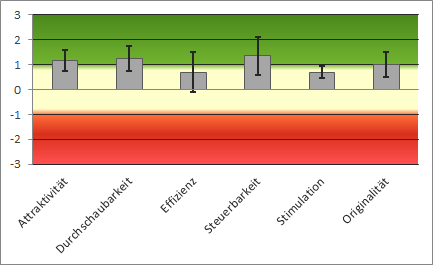
\includegraphics[width=0.55\textwidth,center]{UEQ.png}
\caption{\label{fig:UEQ}Grafische Darstellung der Ergebnisse des UEQs}
\end{figure}

Die Ergebnisse zeigen auf, dass das Hyperaudio"=Plugin in vier Dimensionen knapp ein positives und in zwei Dimensionen ein neutrales Evaluationsergebnis erzielt. Hinsichtlich dieser beiden Dimensionen (Effizienz und Stimulation) sollte das Plugin somit nochmals optimiert werden. Bei Betrachtung der einzelnen Fragebögen scheint Verbesserungspotential bei der Übersichtlichkeit des Plugins zu herrschen, was sich sowohl auf die Effizienz als auch die Durchschaubarkeit negativ auswirkt.
%Außerdem ist erkennbar, dass sich in den Dimensionen Steuerbarkeit und Effizienz eine hohe Varianz ergibt. Dies lässt darauf schließen, dass diese Dimensionen je nach Testkandidat sehr unterschiedlich wahrgenommen werden.

\todo[inline]{Auswertung der Fragen ergänzen}

\subsection{Rolle der Administrierenden}
Auf die Evaluation für die Rolle der Nutzenden sollte nun auch eine Evaluation für die Rolle der Administrierenden folgen. Natürlich könnten hierfür ebenfalls die im vorherigen Abschnitt beschriebene Methode des UEQ durchgeführt werden, es soll nun aber eine weitere Art der Evaluation aufgezeigt werden. Eine alternative Methode stellt das sogenannte Think"=Aloud"=Protokoll beziehungsweise der Think"=Aloud"=Test dar. Bei einem Think"=Aloud"=Test werden die Testkandidaten darum gebeten, das Produkt zu verwenden und währenddessen ihre Gedanken laut auszusprechen \citep{nielsen2012thinking}. \cite{nielsen2012thinking} beschreibt das Vorgehen bei einem Think"=Aloud"=Tests mit den folgenden drei Schritten:

\begin{enumerate}
\item Recruit representative users.
\item Give them representative tasks to perform.
\item Shut up and let the users do the talking.
\end{enumerate}

\todo[inline]{Zitierweise Aufzählung}

Think-Aloud-Tests sind dementsprechend einfach und kostengünstig umsetzbar. Zudem sind sie robust, flexibel, überzeugend und einfach zu erlernen \citep{nielsen2012thinking}. Somit stellt ein Think"=Aloud"=Test eine geeignete Evaluationsmethode für die Rolle der Administrierenden dar.\\
Für die Durchführung eines Think"=Aloud"=Tests für das Hyperaudio"=Plugin müssten zunächst einige Lehrende ausgewählt werden. Diese müssten daraufhin ausgewählte Aufgaben innerhalb des administrativen Bereichs des Hyperaudio"=Plugins erledigen. Hier wäre beispielsweise das Erstellen einer Hyperaudio"=Aktivität in ihrem Kurs denkbar oder auch das Austauschen eines Zusatzinhaltes innerhalb einer Hyperaudio"=Aktivität. Die während des Think"=Aloud"=Tests geäußerten Gedanken der Lehrenden werden festgehalten, um daraus Rückschlüsse bezüglich der Funktionen und Bedienung des Hyperaudio"=Plugins ziehen zu können.



%Definition: In a thinking aloud test, you ask test participants to use the system while continuously thinking out loud — that is, simply verbalizing their thoughts as they move through the user interface.
%https://www.nngroup.com/articles/thinking-aloud-the-1-usability-tool/
%\todo[inline]{Sie sollten dann aber darlegen, wie eine Evaluation mit den Lehrenden aussehen sollte (Ablauf, Fragen, Testinstrumente, Vorgehensweise). Viele Studierende wenden in diesem Kontext das Think aloud protocol an.}

\todo[inline]{Reihenfolge UEQ/Think-Aloud, Nutzende/Administrierende}


\section{Verbesserungsvorschläge}
\label{sec:Verbesserungsvorschlaege}
Im Zuge der Evaluation der Rolle der Nutzenden wurden die Testkandidaten nach dem Ausfüllen des Fragebogens darum gebeten, Wünsche bezüglich funktionaler Erweiterungen des Plugins zu äußern. Die genannten Vorschläge werden im Folgenden in Form von neuen User Stories festgehalten. Für diese User Stories können dieselben Personas (siehe Abschnitt \ref{sec:personas}) verwendet werden wie bereits bei den User Stories aus Abschnitt \ref{sec:UserStories}.
%\todo[inline]{Ich finde es gut, dass Sie Vorschläge zur Verbesserung erbringen. Es ist jedoch unklar, warum Sie erst jetzt auf diese User Stories kommen und diese nicht schon vorher formuliert haben. Die Systematik, mit der Sie diese User Stories ermittelt haben, ist außerdem unklar. Hätten Sie eine Art von Evaluation mit potentiellen Nutzern durchgeführt, wäre Ableitungen dieser Art aus den Evaluationsergebnissen nachvollziehbar,}

\begin{enumerate}[leftmargin=1.3cm,label=US-\arabic*:,ref=US-\arabic*]
\setcounter{enumi}{30}
%\item Als Administrierende möchte Prof. Dr. Karolin Schröder detailliert auf Fehler in der Konfigurationsdatei hingewiesen werden, um solche schneller zu identifizieren, wie beispielsweise Zeitüberschneidungen bei annotierten Zusatzinhalten.
%\item Als Administrierende möchte Prof. Dr. Karolin Schröder Hyperaudio"=Dokumente ganzheitlich innerhalb der Moodle-Umgebung erzeugen können, um nicht mühsam eine Konfigurationsdatei erstellen zu müssen.
%\item Als Administrierende möchte Prof. Dr. Karolin Schröder mehrere Audio-Dateien für Hyperaudio"=Dokumente verwenden können, um die Vertonung von Kurseinheiten in mehreren Abschnitten vornehmen zu können.
%\item Als Administrierende möchte Prof. Dr. Karolin Schröder auch andere Dateiformate als Bilddateien als Zusatzinhalt annotieren, um auch PDF-Dokumente oder Videos einsetzen zu können.
%\item Als Administrierende möchte Prof. Dr. Karolin Schröder noch detailliertere Auswertungen über das Nutzungsverhalten von Hyperaudio"=Dokumenten erhalten, um noch genauere Rückschlüsse über die Stärken und Schwächen des Hyperaudio"=Dokuments zu ermitteln. 
%\item Als Administrierende möchte Prof. Dr. Karolin Schröder verschiedene Audio Cues einsetzen können, um die Studierende auf die verschiedenen Arten von Zusatzinhalten hinzuweisen.
\item \label{US-Kommentar-Bewertung} Als Nutzende möchte Laura Ebert zunächst nur noch die wichtigsten Antworten auf Kommentare angezeigt bekommen, um eine bessere Übersicht bei viel diskutierten Hyperaudio"=Dokumenten zu erhalten.
\item Als Nutzende möchte Laura Ebert nur den Anfang von langen Kommentaren und Notizen angezeigt bekommen, um eine bessere Übersicht im Kommentarbereich zu haben.
\item Als Nutzende möchte Laura Ebert ihrer Notiz eine Datei anfügen, um ihre selbst angefertigte Zeichnung zu hinterlegen.
\item Als Nutzende möchte Laura Ebert Hyperaudio"=Dokumente im Vollbildmodus abspielen können, um die annotierten Zusatzinhalte möglichst groß dargestellt zu bekommen.
%\item Als Nutzende möchte Laura Ebert Kommentare und Antworten löschen und bearbeiten können, um falsche Aussagen entfernen beziehungsweise korrigieren zu können.
\item Als Nutzender möchte Max Lustig, dass der eingegebene Suchbegriff in den gefilterten Kommentaren und Notizen hervorgehoben wird, um die Suchergebnisse schneller bewerten zu können.
\item Als Nutzender wünscht sich Max Lustig eine intelligentere Suchfunktion, um Ergebnisse trotz Schreibfehler oder mit ähnlichen Wörtern zu finden.
\item Als Nutzender möchte Max Lustig nicht nur Zeitpunkte sondern auch Zeitfenster markieren, um Beginn und Ende interessanter Passagen kenntlich zu machen.
\item Als Nutzender möchte Max Lustig schnell vom Kommentarbereich zur Anzeige der Zusatzinhalte springen, sobald ein neuer Zusatzinhalt dargestellt wird, um diesen direkt ohne langes Scrollen einsehen zu können.
\item Als Nutzender möchte Max Lustig über Antworten auf seine Kommentare informiert werden, um nicht proaktiv überprüfen zu müssen, ob jemand seine Fragen beantwortet hat.
\item Als Nutzender möchte Max Lustig die Annotationszeiträume von Zusatzinhalten in der Timeline erkennen können, um einschätzen zu können, wann der nächste Zusatzinhalt dargestellt wird.
\end{enumerate}

\todo[inline]{Notizen aus Gespräch mit Testkandidaten}

Diese zehn neu formulierten User Stories stellen weiterhin nur einen Teil der möglichen User Stories dar. Sie können dennoch als Basis für die Weiterentwicklung des Hyperaudio"=Plugins dienen.

\section{Zusammenfassung}
Bei der Validierung und Evaluation wurde die vorliegende Implementierung des Hyperaudio"=Plugins analysiert. Die Ergebnisse der Validierung zeigen auf, dass bereits viele der formulierten User Stories ermöglicht und entsprechend viele Anforderungen erfüllt wurden. Die durchgeführte Evaluation stellt selbstverständlich keine vollwertige Evaluation des Hyperaudio"=Plugins dar, dennoch konnten bereits Erkenntnisse über die Qualität des Plugins in Bezug auf die User Experience gezogen und entsprechende Stellschrauben ausgemacht werden, die zu einer Verbesserung der UX beitragen können. Zusätzlich wurden Ideen der Testkandidaten zur Verbesserung des Plugins in Form von neuen User Stories festgehalten. Durch die Evaluation konnten diverse Aspekte aufgezeigt werden, welche bei der Weiterentwicklung des Hyperaudio"=Plugins bedacht werden sollten.


%\todo[inline]{{Was Sie beispielsweise nicht evaluiert haben:
%
%nicht-funktionale Anforderungen wie Performanz, Lauffähigkeit auf unterschiedlichen Systemen/Browsern, Usability, User Experience
%
%Können Sie sich drei Leute aus Ihrem persönlichem Umfeld suchen, die einen SUS oder UE Test absolvieren?
%
%UE ist einfach: Rauschenberger, M., Cota, M. P.,  Thomaschewski, J. (2013). Efficient Measurement of the User Experience of Interactive Products. International Journal of Artificial Intelligence and Interactive Multimedia, 2(1), 39–45. http://doi.org/10.9781/ijimai.2013.215
%Es gibt den Fragebogen auf der Webseite und die Werkzeuge zur Auswertung ebenso. 
%
%Außerdem könnten Sie die Technologie Akzeptanz evaluieren: UTAUT, TAM2, TAM ... das sind standardisierte Fragebögen.
%
%Zudem können Sie die Umsetzung der Audio Cues evaluieren und Nutzer schlicht fragen, ob der Ton lauf genug, zur rechten Zeit und eindeutig unterscheidbar erscheint.
%
%Hier sind viele Fragen offen, die in einer wissenschaftlichen Arbeit beantwortet werden sollten. In einer Bachelorarbeit geht es nicht nur darum eine Software zu bauen, sondern auch darum die Anwendung von systematischen Untersuchungsmethoden einzuüben, welche die Nutzbarkeit, Akzeptanz und Zufriedheit der Zielgruppe (zumindest) nahelegt. 
%
%Sie werden natürlich keine hochgradig signifikate Tests durchführen können, dennoch sollte der Wille zur Qualitätssicherung und Verbesserung im wissenschaftlichen Sinne erkenntbar sein.}}